\documentclass[a4paper]{article}
\usepackage[margin=1.5cm]{geometry}
\usepackage{graphicx}
\usepackage{amssymb}
\usepackage{amsmath}
\usepackage{amsfonts}
\usepackage{fontsize}
\changefontsize[12pt]{11pt}
\usepackage{physics}
\newcommand\tab[1][1cm]{\hspace*{#1}}
\usepackage{ulem}

\title{Audio Signal Processing For Guitar Pedal Application}
\author{Aryan Mosavian Pour}

\begin{document}
\maketitle
\section{Equalizer}
Equalizers are comprised of various band pass filters. A band pass filter may be represented in the Fourier domain as
$$H(j\omega) = \text{rect}(\frac{1}{W}(\omega - \omega_0)) + \text{rect}(\frac{1}{W}(\omega + \omega_0))$$
$$h[n] = \mathfrak{F}^{-1}_\text{Discrete}\{H(j\omega)\}(t) = \frac{1}{2\pi}\int_{-\pi}^\pi H(j\omega) e^{-jn\omega}d\omega$$
$$h[n] = \frac{1}{2\pi}\int_{-\pi}^\pi (\Theta(\omega + \omega_0 + \frac{W}{2})-\Theta(\omega - \omega_0 - \frac{W}{2}) + \Theta(\omega - \omega_0 + \frac{W}{2})-\Theta(\omega + \omega_0 - \frac{W}{2}))e^{-jn\omega}d\omega$$
$$h[n] = \frac{1}{2\pi}(\int_{\omega_0 - \frac{W}{2}}^{\omega_0 + \frac{W}{2}} e^{-jn\omega}d\omega + \int_{-\omega_0 - \frac{W}{2}}^{-\omega_0 + \frac{W}{2}} e^{-jn\omega}d\omega)$$
$$h[n] = \frac{1}{2\pi nj}(e^{-jn(\omega_0 + \frac{W}{2})} - e^{-jn(\omega_0 - \frac{W}{2})} + e^{-jn(-\omega_0 + \frac{W}{2})} - e^{-jn(-\omega_0 - \frac{W}{2})})$$
$$h[n] = \frac{1}{2\pi nj}(e^{jn\frac{W}{2}} - e^{-jn\frac{W}{2}})(e^{jn\omega_0} + e^{-jn\omega_0})$$
$$h[n] = \frac{2}{\pi n}\sin(\frac{W}{2} n)\cos(\omega_0 n) = \frac{W}{\pi} \frac{\sin(\frac{W}{2}n)}{\frac{W}{2}n}\cos(\omega_0 n)$$
$$h[n] = \frac{W}{\pi} \text{sinc}(\frac{nW}{2})\cos(\omega_0 n)$$
There are some problems with this solution, though. Most importantly, the system is non-causal. To make it causal, we need to shift our signal and multiply it by some \textit{cropping} function, $c[n]$. 
$$c[n] = \Theta(n + \frac{L}{2}) - \Theta(n - \frac{L}{2})$$
$$h_\text{cropped}[n] = c[n] \times (h[n] * \delta(L/2))$$
There are various types of windows. I will use a square window as it is the simplest.
$$h_\text{cropped}[n] = (\Theta(n + \frac{L}{2}) - \Theta(n - \frac{L}{2})) \frac{W}{\pi} \text{sinc}(\frac{(n-\frac{L}{2})W}{2})\cos(\omega_0 (n-\frac{L}{2}))$$
For my specifications ($\omega_0 = 1300$, $W = 200$) and using $L = 1$, we get the following windowed sinc:
\begin{center}
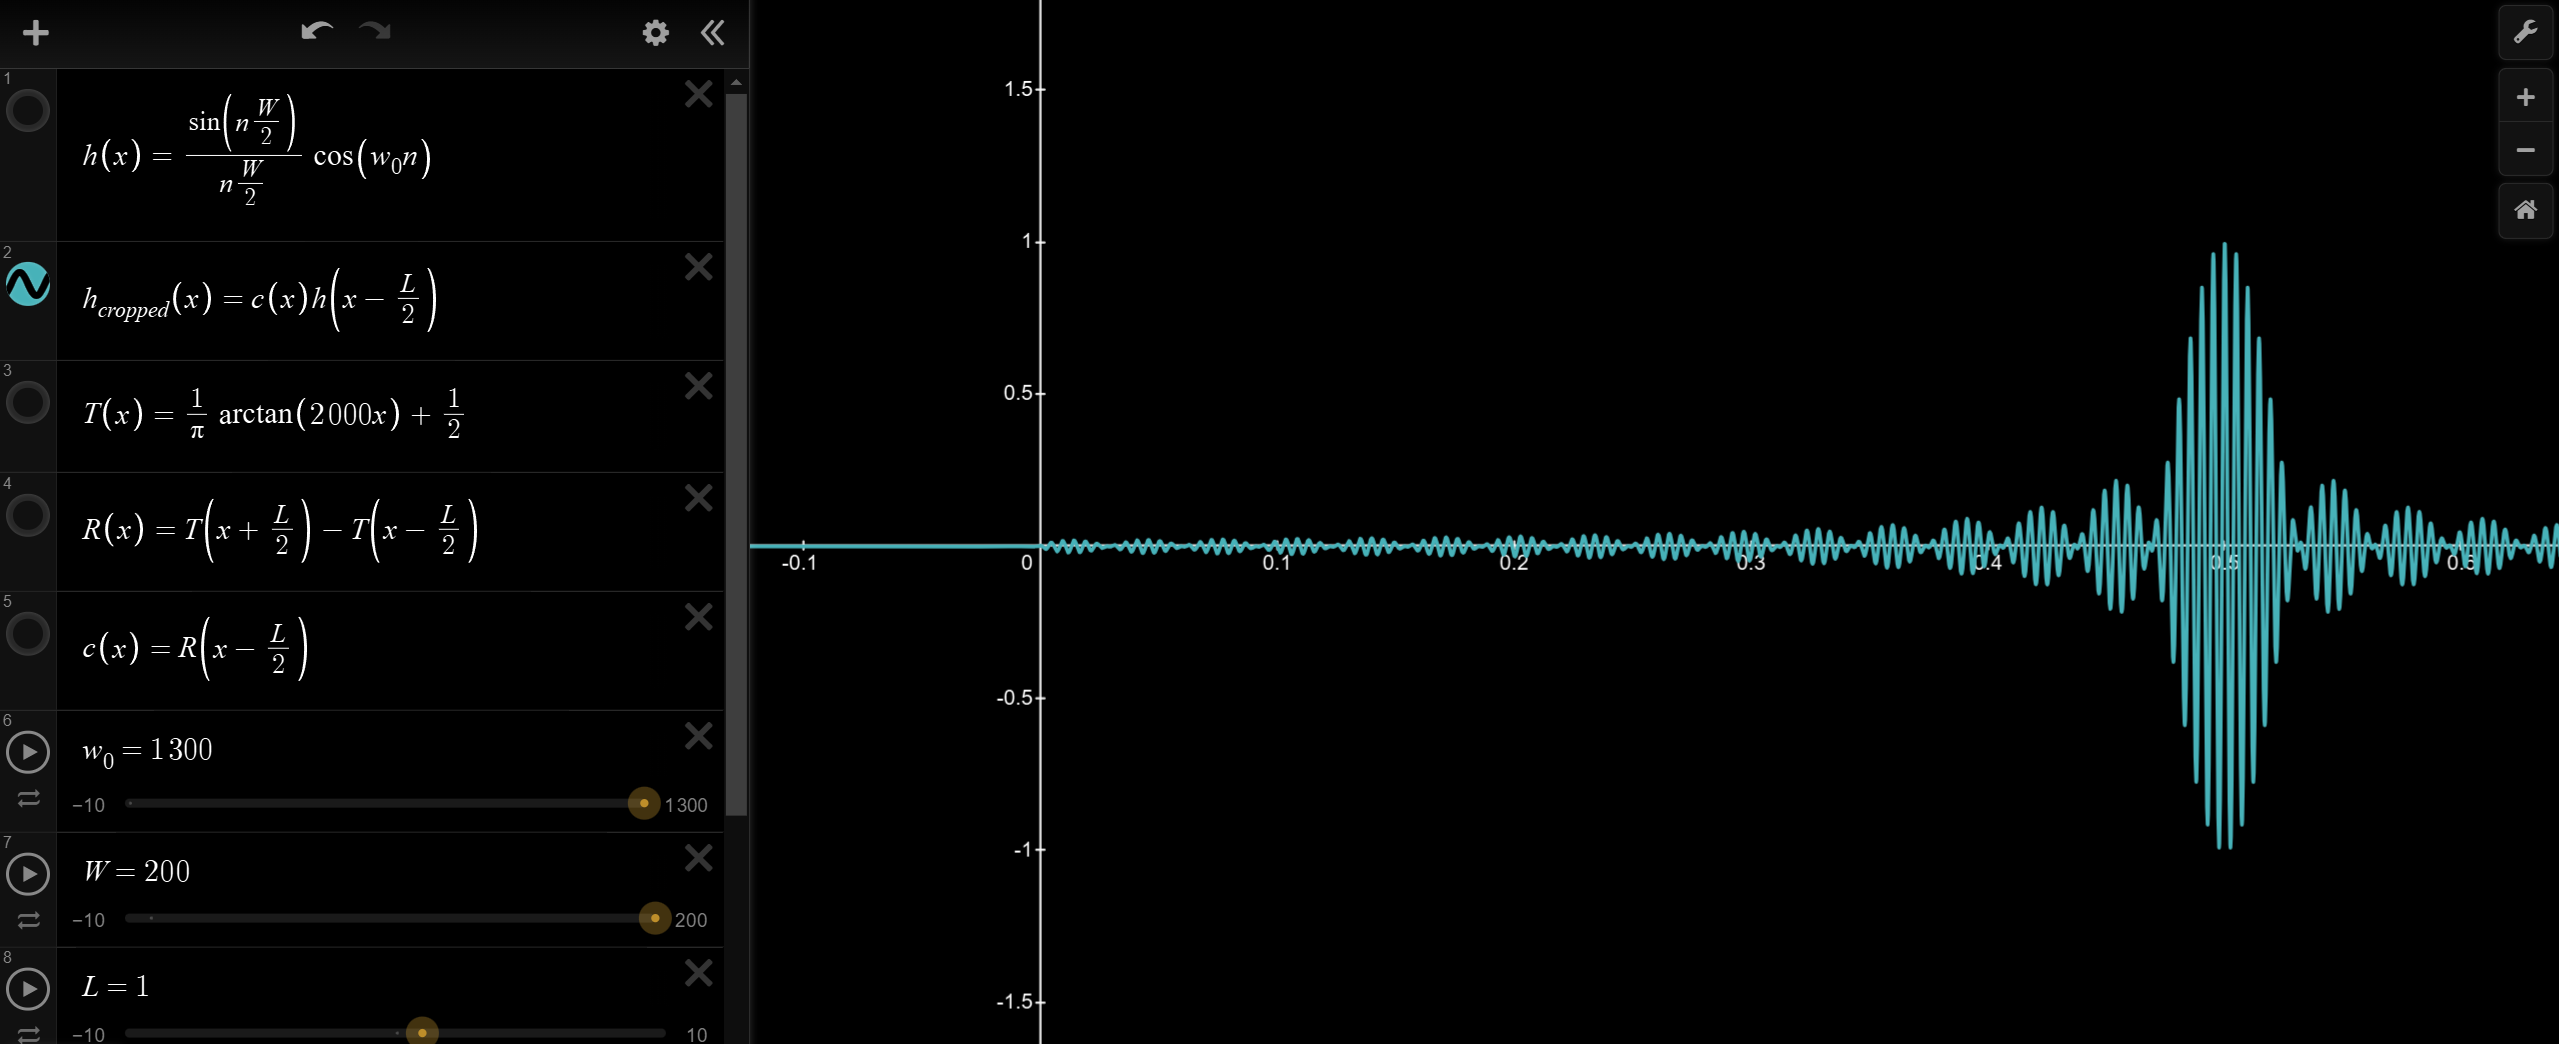
\includegraphics[scale=0.3]{cropped_sinc.png} 
\end{center}
But this introduces yet ANOTHER problem: discontinuities. These greatly affect the frequency response. As a solution, we multiply by a \textit{window} function which effectively smooths out the function. I will use the sine window, $w[n] = \sin(\frac{n\pi}{L})$. We thus get the following function and accompanying graph (with the orange being the cropped function, and the blue being the windowed):
$$h_\text{FIR}[n] = \sin(\frac{n\pi}{L})(\Theta(n + \frac{L}{2}) - \Theta(n - \frac{L}{2})) \frac{W}{\pi} \text{sinc}(\frac{(n-\frac{L}{2})W}{2})\cos(\omega_0 (n-\frac{L}{2}))$$
\begin{center}
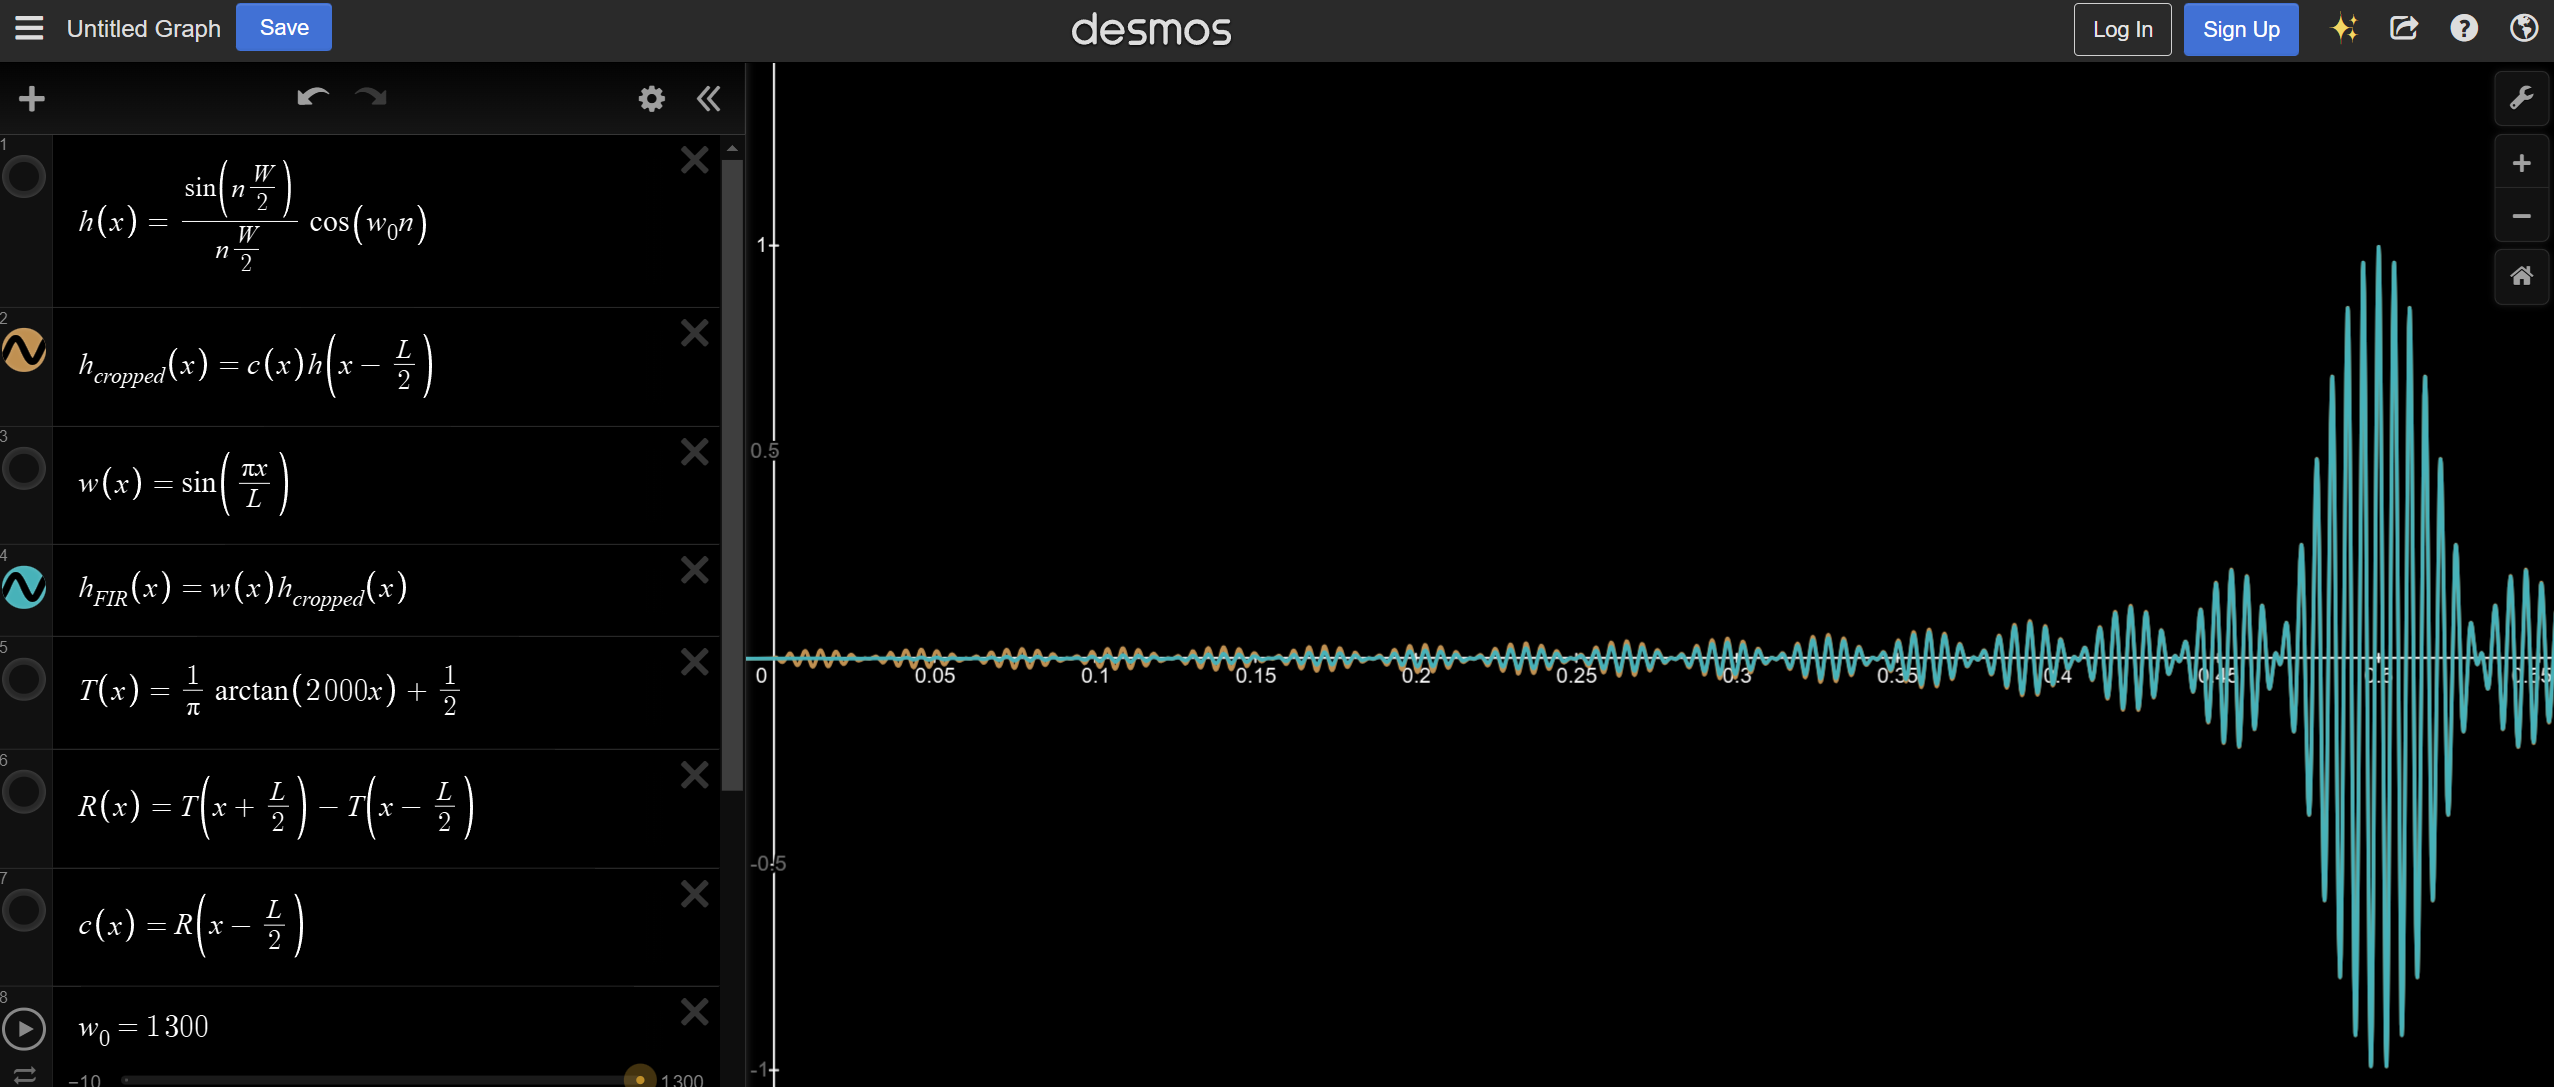
\includegraphics[scale=0.3]{windowed_sinc.png} 
\end{center}
We're now at the finish line: we just need to calculate the output,
$$y[n] = (x * h)[n] := \sum_{m = -M}^M x[n-m]h[m]$$
The final equation representing our system, which is characterized by $\omega_0$ and $W$, is:
$$\boxed{y[n] = \sum_{m = -M}^M x[m]\sin(\frac{n\pi}{L})(\Theta(n + \frac{L}{2}) - \Theta(n - \frac{L}{2})) \frac{W}{\pi} \text{sinc}(\frac{(n-\frac{L}{2})W}{2})\cos(\omega_0 (n-\frac{L}{2}))}$$



























\end{document}